%%% In this section, you will describe all of the various artifacts that you will generate and maintain during the project life cycle. Describe the purpose of each item below, how the content will be generated, where it will be stored, how often it will be updated, etc. Replace the default text for each section with your own description. Reword this paragraph as appropriate.

\subsection{Major Documentation Deliverables}

\subsubsection{Project Charter}
This document will be updated once every week, unless any major change or update occurs. The initial document is set to be submitted on 10/09/2024, Wednesday, and the final document is to be submitted in April 2025.
%Describe how this document will be maintained and updated (how often, under what circumstances, etc.). When will the initial version be delivered? When will the final version be delivered?

\subsubsection{System Requirements Specification}
This document will be updated once every week, unless any major change or update occurs. The initial document is set to be submitted on 10/09/2024, Friday, and the final document is to be submitted in April 2025.
%Describe how this document will be maintained and updated (how often, under what circumstances, etc.). When will the initial version be delivered? When will the final version be delivered?

%\subsubsection{Architectural Design Specification}
%Describe how this document will be maintained and updated (how often, under what circumstances, etc.). When will the initial version be delivered? When will the final version be delivered?

\subsubsection{Detailed Design Specification}
This document will be updated weekly based on progress with the rover and the navigation system. The initial version will be delivered on 10/09/2024 and the final document is to be submitted in April 2025.
%Describe how this document will be maintained and updated (how often, under what circumstances, etc.). When will the initial version be delivered? When will the final version be delivered?

\subsection{Recurring Sprint Items}

\subsubsection{Product Backlog}
The product backlog will be decided as a group vote and will prioritized based on how important it is toward goal of having a educational robot. Github will be used to share the code for the rover. Overleaf and Discord will be used to discuss the rest of what is needed for the rover to function.
%How will items be added to the product backlog from the SRS? How will these items be prioritized? Who makes the decision (product owner, group vote, etc.)? What software will be used to maintain and share the product backlog with team members and stakeholders?

\subsubsection{Sprint Planning}
There will be 9 sprints. Each sprint will be planned based on sprint backlog items and future goals for the rover.
%How will each sprint plan be planned? How many sprints will there be (you need to look at the schedules for this course and previous Senior Design II courses during the appropriate semesters to figure this out).

\subsubsection{Sprint Goal}
The sprint goal will be decided by the group and be discussed as the rover gets built.
%Who decides the sprint goal? How will you involve your customer in this process?

\subsubsection{Sprint Backlog}
The sprint backlog will be decided as a group and will be organized with hardware task and software task. We use github to collaborate on the software and use overleaf and discord to discuss what hardware to focus on.
%Who decides which product backlog items make their way into the sprint backlog? How will the backlog be maintained (collaboration software, a "scrum board", etc.)?

\subsubsection{Task Breakdown}
Tasks will be assigned to team member who volunteer and for the task that are not picked will be given to the members that have enough time and willing to take on the task.
%How will individual tasks be assigned from the sprint backlog? Will it be up to each team member to voluntarily claim a task, or will it come from the product owner? How will time spent on tasks be documented?

%%%%%%%%%%%%%%%%%%%%%%%%%%%%%%%%%%%%%%%%%%%%%%%%%%%%%%%%%%

% \subsubsection{Sprint Burn Down Charts} (REMOVED)
% Who will be responsible for generating the burn down charts for each sprint? How will they be able to access the total amount of effort expended by each individual team member? What format will the burn down chart use (include an example burn down chart below).

%  Be sure to update the image caption (REMOVED)
% \begin{figure}[h!]
%    \centering
%    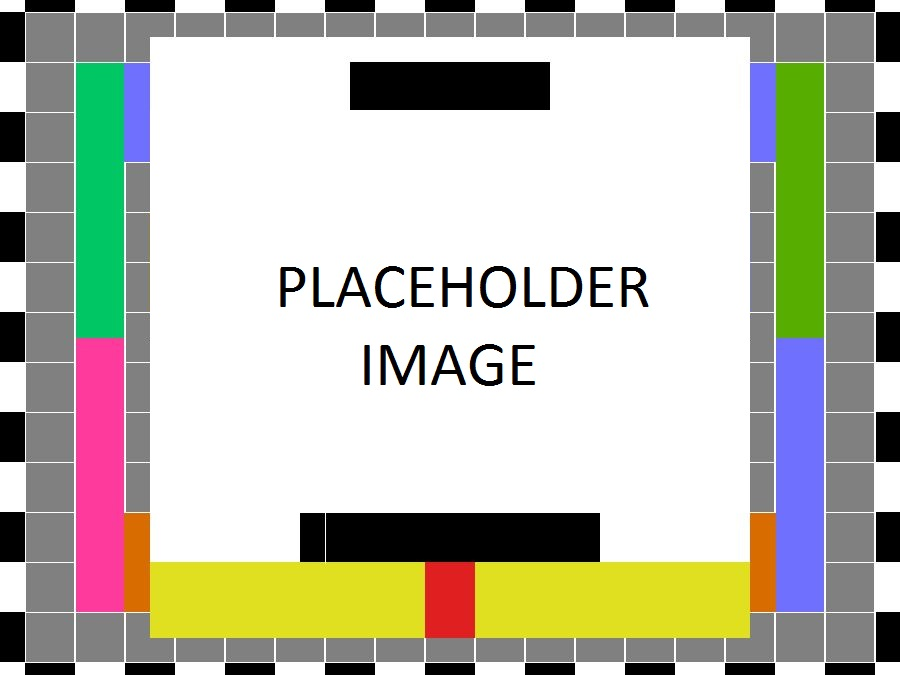
\includegraphics[width=0.5\textwidth]{images/test_image} % Image with a width of half of the text width
%    \caption{Example sprint burn down chart} % Caption - it automatically numbers the figures
% \end{figure}

%%%%%%%%%%%%%%%%%%%%%%%%%%%%%%%%%%%%%%%%%%%%%%%%%%%%%%%%%%

\subsubsection{Sprint Retrospective}
The sprint retrospective will be due on 10/21/2024. We as a team will discuss this after each week on Friday to pull all of our information.
%How will the sprint retrospective be handled as a team? When will this discussion happen after each sprint? What will be documented as a group and as individuals, and when will it be due?

\subsubsection{Individual Status Reports}
Each member will submit a report about their perspective about how the project is going and how each member is contributing. This will be reported after every sprint.
%What sort of status will be reported by each individual member, and how often will it be reported? What key items will be contained in the report?

\subsubsection{Engineering Notebooks}
The engineering notebook will be updated each week by each team member when they are in lab and at the end of each sprint each member would have to have an entry in the notebook. The minimum amount of pages per sprint would be 5 pages. Professor Conly will be the witness for each ENB page. Each member will be held accountable for their own entry.
%How often will the engineering notebook be updated, at a minimum, by each team member? What is the minimum amount of pages that will be completed for each interval, and how long will that interval be? How will the team keep each member accountable? Who will sign of as a "witness" for each ENB page?

\subsection{Closeout Materials}

\subsubsection{System Prototype}
The final system prototype will include a navigation system as well as different components like a pushy arm, sensors and a speaker. The rover will be demonstrated at the end of the spring semester.
%What will be included in the final system prototype? How and when will this be demonstrated? Will there be a Prototype Acceptance Test (PAT) with your customer? Will anything be demonstrated off-site? If so, will there be a Field Acceptance Test (FAT)?

\subsubsection{Project Poster}
The poster will include the rover as well as the many different functions it can do. The dimensions will be 24x32 and will be done by the end of the 4th sprint.
%What will be included on the poster, what will be the final dimensions, and when will it be delivered?

\subsubsection{Web Page}
The project webpage will serve as a key communication tool, showcasing the evolution of our pathfinding algorithms through detailed simulation videos. These videos will demonstrate various versions of our algorithms in action, alongside comparisons to the physical model, providing a clear visualization of performance and accuracy. This will allow users to assess how well the algorithms perform in real-world scenarios and how they improve over time. The webpage will also include a GitHub link, granting access to the project's source code and version history, promoting transparency and enabling collaboration. It will be accessible to the public, allowing stakeholders, potential collaborators, and the wider community to engage with our progress.


\subsubsection{Demo Video}
The demo videos will cover a wide range of topics related to the rover. Such as the key components that allow for different navigation algorithms to be tested on the rover. How to program the rover and what languages are used to do so. The demo video will include b-reel of the rover in action demonstrating different navigation algorithms. Should ideally take around 3-5 mins.

%What will be shown in the demo video(s)? Will you include a B-reel footage for future video cuts? Approximately how long will the video(s) be, and what topics will be covered?

\subsubsection{Source Code}
Our source code will be maintained using GitHub. The project will be open-source under the GPL (GNU General Public License), as many of our pathfinding algorithms (A*, Djikstra, Depth First Search, etc.), are open-source software, to promote transparency.

By adopting the GPL public license, we ensure that the derivations of our source code are open source. The source code including the binaries, will be provided to the customer, to ensure full control over the implementation. The customer can locate the source code via Github, where they have direct access to the repository.  All information containing our licensing will be contained within a readme file at the root of the repository.

\subsubsection{Source Code Documentation}
For code documentation, we will primarily utilize GitHub to ensure version control and collaborative efficiency. In addition, we will use Overleaf for generating our project documentation, which will be published as a downloadable PDF for easy access and distribution. 

\subsubsection{Hardware Schematics}
We will be documenting the connections between the PCB, Sabertooth motor drivers, DC converters, Signal Controllers, and any other component that is added in future sprints.
%Will you be creating printed circuit boards (PCBs) or wiring components together? If so, list each applicable schematic and what sort of data it will contain (PCB layout, wiring diagram, etc.). If your project is purely software, omit this section.

\subsubsection{CAD files}
We plan to use 3D printed parts to add on to the rover. We would be using Blender, Plasticity, or any of the available 3D modeling software.
%Will the project involve any mechanical design, such as 3D printed or laser-cut parts? If so, what software will you use to generate the files and what file formats will you provide in your closeout materials (STL, STEP, OBJ, etc.). If your project is purely software, omit this section.

\subsubsection{Installation Scripts}
The customer will be able to deploy their own navigation system through flashing onto the device by connecting it to the main board. We will provide a basic navigation system to demo the rover's capabilities.
%How will the customer deploy software to new installations? Will you provide installation scripts, install programs, or any other tools to improve the process? Will there be multiple scripts provided (perhaps separate scripts for the graphical front end and back end server software)? 

\subsubsection{ User Manual}
The customer would either need a digital user manual or a physical copy to understand what buttons do what and where extra additions can be placed. 
%Will you customer need a printed or digital user manual? Will they need a setup video? Decide now what will be provided and discuss.
